%% --------------------------------------------------------------
%%
%% N R  S I M U L A T I O N S
%%
%% --------------------------------------------------------------
\begin{frame}{Method} %% ---------- title 
\begin{tikzpicture}[overlay,remember picture]
\uncover<1->{ % <-> |
    \node (t1) [anchor=center,scale=1,opacity=1] at ([shift={(-0.0cm,-0.2cm)}]current page.center){
        \parbox{1.1\textwidth}{
            Key physics: General Relativity, fluid dynamics, radiation transport. 
            \begin{equation*}
                R_{\mu\nu}-\frac{1}{2}Rg_{\mu\nu}=8\pi T_{\mu\nu}, \hspace{5mm} \nabla_{\mu}T^{\mu\nu} = 0, \hspace{5mm} \frac{DF}{Dl}=\mathcal{C}[F], \hspace{5mm} \text{EOS}
            \end{equation*}
            %
            Complex numerical implementation. Expensive simulations. \\
            Numerical relativity codes, \eg, \wisky{} code$^\text{\textcolor{gray}{\citep{Radice:2013apa,Radice:2012cu,Radice:2013xpa,Radice:2013hxh,
                                 Radice:2015nva,Radice:2016dwd,Radice:2018pdn,Radice:2020ids}}}$
            \begin{itemize}
                \item Z4c formulation of $3+1$ decomposed, general relativity,
                %\item Conservative formualtion of relativistic hydrodynamics,
                \item Neutrino radiation transport via Leakage $+$ M0 scheme,
                \item Turbulent viscosity of magnetic origin via GRLES appraoch,
                \item Microphsyical EOS with finite temperature effects.
            \end{itemize}
            Overall, $37$ unique simulations targeted to \GW{}, (some $100+$~ms) % total of $76$,  \\
            % Initial data: constraint equations + Helical killing vector + conformal flatness
            % For free evolution we use z4c: conformal decomposition of the metric fields with improved constraint propagation + dampening (better for non-vacuum spacte time)
            % Moving-puncture gauge (1+log and Gamma-driver) to deal with forming BHs and moving pucntures
            % GRHD is in the conservative formulation, with central, HRSC scheme.
            % Neutrinos are treated with moment formalism, where moment representaiton of Boltzman equation, truncated at (M1 - 2nd moment) with closure achieved via interpolation between otpically thin and thick regimes. 
            % LEackages scheme is na approximation to transport equations that concerns only with the change in leptonic number and loss of energy (no momentum transport or diffusion)
            % EOS: Skyrme model with finite-temperature and composition dependencies (LS220 SLy4) 
            %      Rel.Mean.Field with -//- (DD2 SFh0)
            %      Brueckner-Hartree-Fock extensitions to finite.temp. (BLh)
            % SOftening at very high rho - Lambda-Hyperons or phase transition
            % Numerically: evolution is performed with method of lines and BErger-Oliger algorithm with sub-cycling in time and refluxing 
            % --------
            % Test: L2 norm of the normalized hamiltonian and momentum constraints (vialation)
    }};
}
%
%\uncover<2->{ % <-> |
%    \node (t1) [anchor=center,scale=1,opacity=1] at ([shift={(-0.0cm,-3.6cm)}]current page.center){
%        \parbox{1.1\textwidth}{
%            \textbf{Goal}: Analyzed ejecta/\nuc{}/EM counterparts \& statistical analysis \\
%            \textbf{Methods}: Post-processing pipeline \texttt{bns\_ppr\_tools} for ejecta/disk/remnant
%%            \begin{itemize}
%%            \item Developped post-processing pipeline \texttt{bns\_ppr\_tools}
%%            \item \textbf{Goal}: Analyzed for ejecta/\nuc{}/EM counterparts \& statistical analysis
%%%            \item Statisitcal analysis alongside other models in literature
%%            \end{itemize}
%    }};
%}
\end{tikzpicture}
\end{frame}

%% ----------------------------------------------------------------------------

\begin{frame}{Representative picture of a binary neutron star merger} %% ---------- title 
\begin{tikzpicture}[overlay,remember picture]
    \uncover<1->{ % <-> |
    \node (t1) [anchor=center,scale=1,opacity=1] at ([shift={(-4.1cm,0.5cm)}]current page.center){
        \parbox{0.50\textwidth}{
            % Grav. radiation losses cause the orbital separation to shrink (Softer EOSs -- longer inspiral)
            % Inspiral (${\simeq}10\,$orbits); NSs Zero-temperature, $\beta$-equilibrium \\
            % Merger \& post-merger, $T{\sim}50\,$MeV, $\rho{\sim3.6}\rho_0$. \\
            % Postmerger: Remnant $+$ disk $+$ ejecta; \\
            % Fate: $J$ transport; MHD; $\nu$, GWs \\
            \textbf{System parametrization:} \\
            Tidal interaction 
            % Distrortion of the mass distribution of a given NS in a Grav. Field of another
            % Parametrized with Love Number (computed by solving perturbation of a relativistic star k=f(EOS,Compactness))
            % Combining compactness and Love we get tidal polarizability parameter
            % The dynamics of the two bodies can be described with tidal coupling constant that 
            % describes tidal interaction at leading order
            % Tidal interaction (i) attractive (ii) short range: They accelerate merger, increase frequency
            can be parameterized with \textit{reduced tidal parameter}$^{\text{\textcolor{gray}{\cite{Favata:2013rwa}}}}$
            %
            \begin{equation*}
                \tilde{\Lambda} := \frac{16}{13}\frac{(M_A + 12M_B)M_A^4 \Lambda_A}{M^5}+(A\leftrightarrow B)
            \end{equation*}
            % Gravitational massess are estimated in (conformal, assymptitic? flatness?) in far-field regime and are estimated as integrals over fluid configuration
            %
            $\downarrow\tilde{\Lambda}$ for softer EOS, $\uparrow M$, $\uparrow q=M_A/M_B$ \\
            %
            % A moment of merger is a maximum of the GW amplitude
            %
            % Gauge invariant quantities: Reduced binding energy and angular momentum
            % During the evolution they decrease as GW carry energy away
            % Quasiuniversality: EOS can be captured with $\tilde{\Lambda}$ for equal mass binary
            % 
            % 
    }};
    }
%
    \uncover<1->{ % <-> |
    \node (t1) [anchor=center,scale=1,opacity=1] at ([shift={(3.6cm,0.8cm)}]current page.center){
        \parbox{0.55\textwidth}{
            \textbf{Post-merger state:} \\
            BH, long/short-lived remnants, and disks \\
            % Early postmerger: 
            Core bounces: cold inside, hot interface; shocks at NS surface only \\
            % Right after the merger double-core structure is formed by the two central cores of merging NSs. Cors collide and bounce repeadetly untill they merge. In this process outer layers gain J due to Orbital Angular Momentum Advection and Torques arasing from double-core, non-axisymmetric structure of the sustem. Result: core immersed in low-rho cloud
            % Neutrino burst, ${\sim}15\,$MeV. 
            % Neutrino decouple at different radii
            % Abundance of free $n$, absorbe $\nu_e$, raise $Y_e$; emission of $\bar{\nu}_e$
            % Possible phase transition softens EOS
            % Impact of phase transition depends on density at which it occure
            While cores fuse, remnant shows bar-like deformation \\
            % Main post-merger GW freq. = 2 times dynamical freq.
            % Peaks in GWs associated with hydro mode 
            % Peak frequencies depend on NS prop. -- quasiuniversality
            % Ang. Mom. at merger determines the angular vel. of the bulk of matter
            % Most luminous $\neq$ largest energy
            % Simulations give upper limitof GWs energy
            % GWs backreacts on the fluid, damping the non-axisymmetric modes
            Remnant evolves towards axisymmetry \\
            % Postmerger state: super-Keplerian $J>J_{\rm max}^{\rm equilib}$, $M_b>M_{b \rm, max}^{\rm eqilib}$ -- Highly differential rotation remnant
            % Thermal and neutrino effects $\uparrow$ pressure (${\simeq}10\%$), hence, radius, but not the $M_{\rm max}$. 
            % Rotatin increases NS $M_{\rm max}$ and $R$. 
            % Note: In postmerger $M_{\rm max}^{\rm hot} < M_{\rm max}^{\rm cold}$
            % hence, temperature effects do not stabilize the star.
            % Larger radiuss $\rightarrow$ lower mass-shedding limit
            % Overall: cold classification do not (SMNS, HMNS...) do not apply
            % Magnetic fields can raise $M_{\rm max}$, affecting angular momentum distribution
            % Angular momentum redistribution occures on a viscous time-scale.
            % Inclusion of viscosity show shorter collapse time. 
            % Simulations show a ritational profile with a minimum at the core; as viscous and hydro effects counteract Grav. instabilities in the core, the core will spin up, compactness reduces, hence, the core must shed the excess in angular momentum. Through winds!
            % Neutrinos primarely cool the remnant, removing some of the excess in binding energy. 
            % Simulations show that one-armed instability persists on ${\sim}50\,$ms timescale.
            % Disk $\rho < 10^{13}\,$\gcm
            % Volume integral of the conserved rest-mass density
            % Properties depend on formation
            % formed from matter expelled by tidal torquies at merger 
            % Structure: coled tidal component $+$ hot shocked
            % Nass of the disk may rise as $M_b$ and $J$ are shed by the remnant
            % Shocks ($m=1$) raise entropy, Keplerian, temp profile $\{10,0.1\}$MeV
            % BH formation removes ${\sim}50$ disk
            % Disks around BHs are more compact and hotter
            % In case of PC, $q=1$ binaries give little disk, while $q{\simeq}1.4$ result in more massive disks. Hiher $q$ lead to tidal disruption of a compantion and formation of a massive cold disk.
            % In high $q$ cases tidal tail falls back, disturbing the disk
            % -------
            % Constraints on NS mass and radius can come from NICER, XMM, NANOGrav, of pulsars and LVC of GW170817
            % Disk formation After merger, anguilar momentum is transfered from inner to the outer layers causing outer layers to expand (and it will remain outside the ISCO when BH forms). 
            % In prompt collapse cases the disk expected to be smaller as there is no angular momentum transport due to turbulence. Only external and low density outer layers of the star are able to gaun enough angular momentum die to tidal torques and pushed away from the bulk of the merging stars. 
            % Soft EOS remnant cannot hold high J by tidal torques. 
    }};
    }

    \uncover<1->{ % <-> |
        \node (img1) [anchor=center,scale=1,opacity=1] at ([shift={(-1.cm,-2.8cm)}]current page.center){
            \parbox{1.0\textwidth}{
                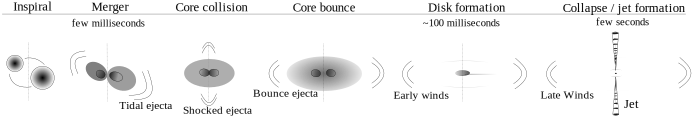
\includegraphics[height=2.7cm]{figures/bns_evolution_transparent.pdf}
                %            \hspace*{10mm} Density modes in the remnant 
                %Modes analysis for exemplary equal-mass long-live and short-lived
                %        remnants. The evolution of the $m=2$ and the $m=1$ monitored by
                %        Eq.~\eqref{eq:modes} is shown for the DD2 and LS220 remnant with and
                %        without turbulent viscosity. The $m=2$ mode in the long-lived
                %        remnant is strongly damped by the emission of gravitational
                %        radiation and becomes comparable to the $m=1$ mode on a timescale of
                %        ${\gtrsim}20\,$ms. Turbulent viscosity sustain the $m=2$ mode for
                %        a longer period. The $m=2$ mode is instead dominant to collapse in
                %        the short-lived remnant.
                %        (Adopted from \cite{Nedora:2020pak})
        }};
    }
\end{tikzpicture}
\end{frame}

%% -------------------------- H Y D R O  M O D E S --------------------------------
%% FROM LETTER 

%From the fluid's stress energy tensor,
%we compute the angular momentum density flux $J_r = T_{ra}(\partial_\phi)^a$,
%where $\phi$ is the cylindrical angular coordinate;
%angular momentum is conserved if $(\partial_\phi)^a$ is a Killing vector.
%
%% FROM PAPER 

%The fluid's angular momentum analysis in the remnant and disk is performed
%assuming axisymmetry,
%%(see Appendix~\ref{app:ang} for derivation)
%that is, we assume $\phi^{\mu} = (\partial_{\phi})^{\mu}$ is a Killing
%vector. Accordingly, the conservation law (Eq.~\eqref{eq:theory:tmunu_eq_0}) 
%reads
%%
%\begin{equation}
%\partial_t(T^{\mu\nu}\phi_{\nu}n_{\nu}\sqrt{\gamma}) -
%\partial_i(\alpha T^{i \nu}\phi_{\nu}\sqrt{\gamma}) = 0 \ ,
%\end{equation}
%%
%where $n^\mu$ is the normal vector to the spacelike hypersurfaces of
%the spacetime's $3+1$ decomposition.
%%
%The equation implies the conservation of the angular momentum 
%\begin{equation}
%J = % \int j dV = 
%%- \int \, T_{\mu\nu}n^{\mu}\phi^{\nu}\,\dd ^3x = 
%-\int \,
%T_{\mu\nu}n^{\mu}\phi^{\nu}\,\sqrt{\gamma}\, \dd^3 x\ .
%\end{equation}
%%
%In the cylindrical coordinates $x^i=(r,\phi,z)$ adapted to the symmetry
%the angular momentum density is  
%%
%\begin{equation}
%j = %-
%\rho h W^2 v_{\phi} \ ,
%\label{eq:method:ang_mom}
%\end{equation}
%%
%and the angular momentum flux is 
%%
%\begin{equation}
%\alpha\sqrt{\gamma}T^r _{\nu}\phi^{\nu} =
%\alpha\sqrt{\gamma}\rho h W^2 (v^{r}v_{\phi}) .
%\end{equation}
%
%We evaluate these quantities from the 3D snapshots of our simulations.
%\begin{frame}{Post-merger remnant dynamics$^\text{\textcolor{gray}{\citep{Nedora:2019jhl,Nedora:2020pak}}}$} %% ---------- title 
%
%    \begin{tikzpicture}[overlay,remember picture]
%        %% ---------------------- Density Modes -----------------------------
%        \uncover<1-2>{ % <-> |
%            \node (t1) [anchor=center,scale=1,opacity=1] at ([shift={(-3.6cm,1.5cm)}]current page.center){
%                \parbox{0.6\textwidth}{
%                    \textbf{Density modes:} decomposition in Fourier modes $e^{-i m\phi}$ 
%                    of the Eulerian rest-mass density 
%                    %\vspace{-3mm}
%                    \begin{equation*}
%                        \label{eq:modes}
%                        C_m(t) = \int \rho(x,y,z=0,t) e^{-i m \phi(x,y)} \text{d}x \text{d} y \, ,
%                    \end{equation*}
%                    % Non-axysimmetric oscillation modes of the remnant persist
%            }};
%        }
%        % ------------------- Angular momentum ----------------------------
%        \uncover<3-5>{ % <-> |
%            \node (t1) [anchor=center,scale=1,opacity=1] at ([shift={(-3.6cm,1.7cm)}]current page.center){
%                \parbox{0.6\textwidth}{
%                    \textbf{The angular momentum flux} in the cylindrical coordinates % $x^i=(r,\phi,z)$.
%                    % $\phi^{\nu}$ is the generator of the rotations in the orbital plane.
%                    (assuming axial symmetry).
%                    %\vspace{-3mm}
%                    \begin{equation*}
%                        \alpha\sqrt{\gamma}T^r _{\nu}\phi^{\nu} =
%                        \alpha\sqrt{\gamma}\rho h W^2 (v^{r}v_{\phi})\, ,
%                    \end{equation*}
%                    % assiming $\phi^{\mu} = (\partial_{\phi})^{\mu}$ is a Killing vector. % angular momentum is conserved
%            }};
%        }
%        %
%        % ----------------------- F I G U R E S -------------------------------
%        %
%        \uncover<1-2>{ % <-> |
%            \node (img1) [anchor=center,scale=1,opacity=1] at ([shift={(4.5cm,-0.6cm)}]current page.center){
%                \parbox{0.5\textwidth}{
%                    \includegraphics[height=6.4cm]{phd_figs/remnant/dens_modes/modes_rho_dd2.pdf}
%                    \hspace*{10mm} Density modes in the remnant 
%                    %Modes analysis for exemplary equal-mass long-live and short-lived
%                    %        remnants. The evolution of the $m=2$ and the $m=1$ monitored by
%                    %        Eq.~\eqref{eq:modes} is shown for the DD2 and LS220 remnant with and
%                    %        without turbulent viscosity. The $m=2$ mode in the long-lived
%                    %        remnant is strongly damped by the emission of gravitational
%                    %        radiation and becomes comparable to the $m=1$ mode on a timescale of
%                    %        ${\gtrsim}20\,$ms. Turbulent viscosity sustain the $m=2$ mode for
%                    %        a longer period. The $m=2$ mode is instead dominant to collapse in
%                    %        the short-lived remnant.
%                    %        (Adopted from \cite{Nedora:2020pak})
%            }};
%        }
%        \uncover<3-5>{ % <-> |
%            \node (img1) [anchor=center,scale=1,opacity=1] at ([shift={(5.3cm,-0.6cm)}]current page.center){
%                \parbox{0.5\textwidth}{
%                    \includegraphics[height=6cm]{phd_figs/raycasting_smooth_cropped.pdf}
%                    
%                    \hspace*{2.8mm}Spiral arms within the disk
%            }};
%        }
%%        \uncover<4-4>{ % <-> |
%%            \node (img2) [anchor=center,scale=1,opacity=1] at ([shift={(4.2cm,-0.4cm)}]current page.center){
%%                \parbox{0.5\textwidth}{
%%                    \includegraphics[height=6.0cm]{phd_figs/remnant/evol_jflux_2d_DD2_M13641364_M0_SR_R1.pdf}
%%                    
%%                    \hspace*{2.8mm}Ang. mom. transport through disk
%%            }};
%%        }
%        %
%        % ------------------------- N O T E S -----------------------------
%        %
%        \uncover<2-2>{ % <-> |
%            \node (t2) [anchor=center,scale=1,opacity=1] at ([shift={(-3.8cm,-1.5cm)}]current page.center){
%                \parbox{0.6\textwidth}{
%                    \begin{itemize}
%                        \item Post-merger remnant is not axisymmetric
%                        \item bar-shaped, $m=2$ is dominant at the start, dumped by \acp{GW}
%                        \item one-armed, $m=1$, ramaines till ${\sim}100$~ms$^\text{\textcolor{gray}{\citep{Radice:2016gym,East:2016zvv}}}$
%                        \item $m=1$ mode is stronger if \mr{} is higher
%                        %                        \item Bar-shaped $m=2$ dominats the \textbf{early} phase
%                        %                        and later $m=2$ is damped by the emission of \acp{GW}
%                    \end{itemize}
%            }};
%        }
%        % -------------------------------------------------------------
%        \uncover<4-5>{ % <-> |
%            \node (t2) [anchor=center,scale=1,opacity=1] at ([shift={(-3.8cm,-0.cm)}]current page.center){
%                \parbox{0.6\textwidth}{
%                    \begin{itemize}
%                        \item Shocks and tidal torques affect the disk, 
%                        Injecting mass, energy, angular momentum.
%                        \item spiral arms is a generic hydrodynamic effect.
%                        % exerted from non-axisymmetric remnant $\rightarrow$ disk;
%                    \end{itemize}
%            }};
%        }
%        % ---------------------------------------------------------
%        \uncover<5-5>{ % <-> |
%            \node (t2) [anchor=center,scale=1,opacity=1] at ([shift={(-3.8cm,-2.8cm)}]current page.center){
%                \parbox{0.6\textwidth}{
%                    \begin{itemize}
%                        %\item The $J$ is transported via spiral waves induced by $m=\{1,2\}$ modes.
%                        \item Spiral density modes inject ${\sim}0.1-0.4\,\Msun$ and ${\sim}50\%$ of remnant's angular momentum into the disk
%                        \item Accretion, mass-shedding, weak processes
%                    \end{itemize}
%            }};
%        }
%    %}
%    %shocks are generated at the collisional interface of the \acp{NS} cores,
%    %as well as, tidal torques exerted by the non axisymmetric remnant result in a formation
%    %of the disk.
%    %Matter, energy and angular momentum are injected into the disk as the spiral 
%    %density waves propagate outwards from the mass-shedding \ac{MNS} remnant
%    \end{tikzpicture}
%    %\begin{itemize}
%    %    \item Not axisymmetric. Angular momentum redistribution, \acp{GW} losses %\cite{Bernuzzi:2015opx,Radice:2018xqa}
%    %    \item Long-term evolution driven by viscous processes \& weak interactions
%    %    \item After \ac{GW} losses \ac{MNS} have excess in $M$ with respect to the cold, rigid.rot equilibria %\citep{Radice:2018xqa}.
%    %    \item \ac{MNS} remnant evolves towards stability at the mass-shedding limit
%    %    \item Collapse to a \ac{BH} depends on post-merger state, temperature and composition
%    %\end{itemize}
%    %
%    %\begin{figure}[t]
%    %    \centering
%    %    \includegraphics[width=0.49\textwidth]{raycasting_smooth_cropped.pdf}
%    %    \caption{3D distribution of angular momentum density flux $J_r$
%        %        from the DD2 simulation with turbulent viscosity at ${\sim}43.5$~ms after
%        %        merger. $J_r$ is shown on a central region of
%        %        $(89\times89\times60)$~km${}^3$ covering the remnant NS
%        %        and disk, and it is given in units where $c=G=\Msun=1$.
%        %        (Adapted from \citet{Nedora:2019jhl})
%        %    }
%    %    \label{fig:ang_mom_flux}
%    %\end{figure}
%    %
%    %\begin{itemize}
%    %    \item High $q$ models undergo prompt collapse (no core bounce) % central density monotonically rises\citep{Radice:2020ddv,Bernuzzi:2020tgt,Bernuzzi:2020txg}. 
%    %    \item 
%    %\end{itemize}
%\end{frame}



































%\begin{frame}{Hydrodynamic modes in the \pmerg{} remnant$^\text{\textcolor{gray}{\citep{Nedora:2019jhl,Nedora:2020pak}}}$} %% ---------- title 
%    
%    \begin{tikzpicture}[overlay,remember picture]
%        
%        \uncover<1->{ % <-> |
%            \node (t1) [anchor=center,scale=1,opacity=1] at ([shift={(-3.6cm,1.5cm)}]current page.center){
%                \parbox{0.6\textwidth}{
%                    Decomposition in Fourier modes $e^{-i m\phi}$ 
%                    of the Eulerian rest-mass density 
%                    \begin{equation*}
%                        \label{eq:modes}
%                        C_m(t) = \int \rho(x,y,z=0,t) e^{-i m \phi(x,y)} \text{d}x \text{d} y \, ,
%                    \end{equation*}
%                % Non-axysimmetric oscillation modes of the remnant persist
%            }};
%        }
%        %
%        \uncover<1->{ % <-> |
%            \node (img1) [anchor=center,scale=1,opacity=1] at ([shift={(4.5cm,-0.6cm)}]current page.center){
%                \parbox{0.5\textwidth}{
%                    \includegraphics[height=6.4cm]{phd_figs/remnant/dens_modes/modes_rho_dd2.pdf}
%                    \hspace*{10mm} Density modes in the remnant 
%                    %Modes analysis for exemplary equal-mass long-live and short-lived
%                    %        remnants. The evolution of the $m=2$ and the $m=1$ monitored by
%                    %        Eq.~\eqref{eq:modes} is shown for the DD2 and LS220 remnant with and
%                    %        without turbulent viscosity. The $m=2$ mode in the long-lived
%                    %        remnant is strongly damped by the emission of gravitational
%                    %        radiation and becomes comparable to the $m=1$ mode on a timescale of
%                    %        ${\gtrsim}20\,$ms. Turbulent viscosity sustain the $m=2$ mode for
%                    %        a longer period. The $m=2$ mode is instead dominant to collapse in
%                    %        the short-lived remnant.
%                    %        (Adopted from \cite{Nedora:2020pak})
%            }};
%        }
%        
%        \uncover<1->{ % <-> |
%            \node (t2) [anchor=center,scale=1,opacity=1] at ([shift={(-3.8cm,-1.8cm)}]current page.center){
%                \parbox{0.6\textwidth}{
%                    \begin{itemize}
%                        \item Newly born remnant is not axisymmetric
%                        \item Bar-shaped $m=2$ dominats the \textbf{early} phase
%                        and later $m=2$ is damped by the emission of \acp{GW}
%                        \item One-armed $m=1$ is present on ${\sim}100$~ms 
%                        \item $m=1$ mode is stronger if \mr{} is higher
%                        \item And as the $m=1$ modes are not efficiently damped$^\text{\textcolor{gray}{\citep{Paschalidis:2015mla,Radice:2016gym,Lehner:2016wjg,East:2016zvv}}}$
%                    \end{itemize}
%            }};
%        }
%
%\end{tikzpicture}
%%\begin{itemize}
%%    \item Not axisymmetric. Angular momentum redistribution, \acp{GW} losses %\cite{Bernuzzi:2015opx,Radice:2018xqa}
%%    \item Long-term evolution driven by viscous processes \& weak interactions
%%    \item After \ac{GW} losses \ac{MNS} have excess in $M$ with respect to the cold, rigid.rot equilibria %\citep{Radice:2018xqa}.
%%    \item \ac{MNS} remnant evolves towards stability at the mass-shedding limit
%%    \item Collapse to a \ac{BH} depends on post-merger state, temperature and composition
%%\end{itemize}
%%
%%\begin{figure}[t]
%%    \centering
%%    \includegraphics[width=0.49\textwidth]{raycasting_smooth_cropped.pdf}
%%    \caption{3D distribution of angular momentum density flux $J_r$
%%        from the DD2 simulation with turbulent viscosity at ${\sim}43.5$~ms after
%%        merger. $J_r$ is shown on a central region of
%%        $(89\times89\times60)$~km${}^3$ covering the remnant NS
%%        and disk, and it is given in units where $c=G=\Msun=1$.
%%        (Adapted from \citet{Nedora:2019jhl})
%%    }
%%    \label{fig:ang_mom_flux}
%%\end{figure}
%%
%%\begin{itemize}
%%    \item High $q$ models undergo prompt collapse (no core bounce) % central density monotonically rises\citep{Radice:2020ddv,Bernuzzi:2020tgt,Bernuzzi:2020txg}. 
%%    \item 
%%\end{itemize}
%\end{frame}
%
%%% ----------------------------------------
%
%
%
%
%%% ----------------------------------------------------------------
%%%
%%% Spiral Arms
%%%
%%% ----------------------------------------------------------------
%
%\begin{frame}{Spiral arms in \pmerg{} remnant$^\text{\textcolor{gray}{\citep{Nedora:2019jhl}}}$} %% ---------- title 
%\begin{tikzpicture}[overlay,remember picture]
%\uncover<1->{ % <-> |
%    \node (t1) [anchor=center,scale=1,opacity=1] at ([shift={(-3.2cm,1.2cm)}]current page.center){
%        \parbox{0.65\textwidth}{
%            The angular momentum flux in the cylindrical coordinates.% $x^i=(r,\phi,z)$.
%            % $\phi^{\nu}$ is the generator of the rotations in the orbital plane.
%            \begin{equation*}
%            \alpha\sqrt{\gamma}T^r _{\nu}\phi^{\nu} =
%            \alpha\sqrt{\gamma}\rho h W^2 (v^{r}v_{\phi})\, ,
%            \end{equation*}
%            assiming $\phi^{\mu} = (\partial_{\phi})^{\mu}$ is a Killing vector. % angular momentum is conserved
%    }};
%}
%
%\uncover<1-1>{ % <-> |
%    \node (img1) [anchor=center,scale=1,opacity=1] at ([shift={(5.3cm,-0.6cm)}]current page.center){
%        \parbox{0.5\textwidth}{
%            \includegraphics[height=6cm]{phd_figs/raycasting_smooth_cropped.pdf}
%            
%            \hspace*{2.8mm}Spiral arms within the disk
%    }};
%}
%
%%shocks are generated at the collisional interface of the \acp{NS} cores,
%%as well as, tidal torques exerted by the non axisymmetric remnant result in a formation
%%of the disk.
%%Matter, energy and angular momentum are injected into the disk as the spiral 
%%density waves propagate outwards from the mass-shedding \ac{MNS} remnant
%\uncover<1->{ % <-> |
%    \node (t2) [anchor=center,scale=1,opacity=1] at ([shift={(-3.5cm,-1.8cm)}]current page.center){
%        \parbox{0.6\textwidth}{
%            \begin{itemize}
%                \item Shocks and tidal torques exerted from non-axisymmetric remnant $\rightarrow$ disk;
%                \item spiral arms is a generic hydrodynamic effect.
%            \end{itemize}
%            Injection of matter, energy and angular momentum.
%    }};
%}
%
%\end{tikzpicture}
%
%\end{frame}
%
%
%%% ----------------------------------------------------------------
%%%
%%% Angular momentum trasport
%%%
%%% ----------------------------------------------------------------
%
%\begin{frame}{Angular momentum transport in \pmerg{} remnant$^\text{\textcolor{gray}{\citep{Nedora:2020pak}}}$} %% ---------- title 
%
%\begin{tikzpicture}[overlay,remember picture]
%
%\uncover<1->{ % <-> |
%    \node (img2) [anchor=center,scale=1,opacity=1] at ([shift={(4.2cm,-0.4cm)}]current page.center){
%        \parbox{0.5\textwidth}{
%            \includegraphics[height=6.0cm]{phd_figs/remnant/evol_jflux_2d_DD2_M13641364_M0_SR_R1.pdf}
%            
%            \hspace*{2.8mm}Ang. mom. transport through disk
%    }};
%}
%%shocks are generated at the collisional interface of the \acp{NS} cores,
%%as well as, tidal torques exerted by the non axisymmetric remnant result in a formation
%%of the disk.
%%Matter, energy and angular momentum are injected into the disk as the spiral 
%%density waves propagate outwards from the mass-shedding \ac{MNS} remnant
%
%\uncover<1->{ % <-> |
%    \node (t2) [anchor=center,scale=1,opacity=1] at ([shift={(-3.8cm,-0.8cm)}]current page.center){
%        \parbox{0.6\textwidth}{
%            \begin{itemize}
%                \item The $J$ is transported via spiral waves induced by $m=\{1,2\}$ modes.
%                \item Spiral density modes inject ${\sim}0.1-0.4\,\Msun$ into the disk
%                \item ${\sim}50\%$ of $J$ remnant $\rightarrow$ disk
%                \item Mass injection is stronger in models with stiffer EOS. 
%                \item Accretion, mass-shedding, weak processes
%                % \item Larger temperatures lead to lower rotational frequency at which the mass 
%                % shedding occurs% \citep{Kaplan:2013wra}. 
%            \end{itemize}
%    }};
%}
%
%\end{tikzpicture}
%
%\end{frame}











%% ----------------------------------------------------------------
%%
%% Long-term Evolution
%%
%% ----------------------------------------------------------------



\begin{frame}{Long term evolution \& remnant's fate$^\text{\textcolor{gray}{\citep{Nedora:2020pak}}}$} %% ---------- title 

%As the disk expands and cools, the recombination of nucleons into alpha particles 
%starts to take place. The energy, released in recombination, might be sufficient 
%for the outermost layers to become unbound, generating an outflow and contributing 
%to the disk depletion \citep{Beloborodov:2008nx,Lee:2009uc,Fernandez:2013tya}.
%%
%This process however is expected to take place on timescales, longer than
%those that are simulated here. On the $\sim100$~ms timescale, however, the outflows 
%are driven by the neutrino heating, above the remnant, the so-called neutrino-driven 
%wind (\nwind; \citep{Dessart:2008zd,Perego:2014fma,Just:2014fka}), and by the dynamical 
%interactions between the \ac{MNS} remnant and the disk, the \swind{} \citep{Nedora:2019jhl}.
%%
%We discuss the properties of the \nwind{} found in our simulations
%in Sec.~\ref{sec:bns_sims:nwind} and the properties of the 
%\swind{} in Sec.~\ref{sec:bns_sims:sww}.

\begin{tikzpicture}[overlay,remember picture]

%We evaluate the amount of angular momentum lost to \acp{GW} following the 
%\citet{Damour:2011fu,Bernuzzi:2012ci,Bernuzzi:2015rla}\footnote{
%    The radiated angular momentum is computed from the 
%    multipole loments $N_{lm}$ for the \ac{NR} complex "news function" at infinity. 
%    The $J_{z;\text{rad}}(t)$ is computed as \citep{Damour:2011fu} 
%    \begin{equation*}
%    \Delta J_{z\text{rad}}(t) \frac{1}{16}\sum_{l,m}^{l_{max}}\int_{t_0}^{t} dt' m \mathcal{L}[h_{lm}(t')(N_{lm}(t'))^*],
%    \end{equation*}
%    where $h_{lm}$ is the multipolar metric waveform, 
%    $N_{lm}(t) = dh_{lm}(t) / dt$, the news function, and $l_{max}=8$.
%    The $J$ loss is metric dependent ($h$).
%    The $h$ (strain???) is computed from $\Psi_4(t) = dN/dt = d^2h/dt^2$ by a 
%    frequency-domain integration procedure with a low-frequency cut 
%    $\omega_0 = 0.032/(m_1+m_2)$.
%    The routines used for the calculation are taken from the scientific library
%    \texttt{scidata}, available at \url{https://bitbucket.org/dradice/scidata}.
%}.

\uncover<1->{ % <-> |
    \node (t1) [anchor=center,scale=1,opacity=1] at ([shift={(-3.4cm,1.2cm)}]current page.center){
        \parbox{0.65\textwidth}{
            Fourier mode decomposition $e^{-i m\phi}$ of the Eulerian rest-mass density 
            %Modes analysis for exemplary equal-mass long-live and short-lived
            %                    %        remnants. The evolution of the $m=2$ and the $m=1$ monitored by
            %                    %        Eq.~\eqref{eq:modes} is shown for the DD2 and LS220 remnant with and
            %                    %        without turbulent viscosity. The $m=2$ mode in the long-lived
            %                    %        remnant is strongly damped by the emission of gravitational
            %                    %        radiation and becomes comparable to the $m=1$ mode on a timescale of
            %                    %        ${\gtrsim}20\,$ms. Turbulent viscosity sustain the $m=2$ mode for
            %                    %        a longer period. The $m=2$ mode is instead dominant to collapse in
            %                    %        the short-lived remnant.
            %                    %        (Adopted from \cite{Nedora:2020pak})
            \begin{itemize}
                \item Newly born remnant is not axisymmetric, $m=2$, $m=1$ modes most prominent; 
                \item One-armed $m=1$ is present on ${\sim}100$~ms 
                \item Matter, energy and angular momentum injected
                %                        \item Bar-shaped $m=2$ dominats the \textbf{early} phase
                %                        and later $m=2$ is damped by the emission of \acp{GW}
                %                        \item One-armed $m=1$ is present on ${\sim}100$~ms 
                %                        \item $m=1$ mode is stronger if \mr{} is higher
                %                        \item And as the $m=1$ modes are not efficiently damped$^\text{\textcolor{gray}{\citep{Paschalidis:2015mla,Radice:2016gym,Lehner:2016wjg,East:2016zvv}}}$
                %%    \item Not axisymmetric. Angular momentum redistribution, \acp{GW} losses %\cite{Bernuzzi:2015opx,Radice:2018xqa}
                %%    \item Long-term evolution driven by viscous processes \& weak interactions
                %%    \item After \ac{GW} losses \ac{MNS} have excess in $M$ with respect to the cold, rigid.rot equilibria %\citep{Radice:2018xqa}.
                %%    \item \ac{MNS} remnant evolves towards stability at the mass-shedding limit
                %%    \item Collapse to a \ac{BH} depends on post-merger state, temperature and composition
                %\begin{itemize}
                    %                \item Shocks and tidal torques exerted from non-axisymmetric remnant $\rightarrow$ disk;
                    %                \item spiral arms is a generic hydrodynamic effect.
                    %            \end{itemize}
                %            Injection of matter, energy and angular momentum.
            \end{itemize}
    }};
}
\uncover<2->{ % <-> |
    \node (t1) [anchor=center,scale=1,opacity=1] at ([shift={(-3.4cm,-2.5cm)}]current page.center){
        \parbox{0.65\textwidth}{
            \begin{itemize}
                % Viscosity foces rotating equilibria to rotate rigidly
                % Non-axial symmetry -- gravitational radiation
                % ADM mass and angular momentum must be conserved 
                % J_GW is computed from the Weil scalar (Psi4) decomposed into s=-2 spin-weighted spherical harmonics
                % Angular momentum, trasported away by GWs
                % Differential rotation is reduced by the non-axisymmetric torques and GWs losses that redistribute angular momentum from inner to the outer regions
                \item Remnant is born with excess in baryonic mass, $M_b$, and angular momentum, $J$, (HMNS)
                % \item \acp{GW} remove some $J$
                \item Angular momentum is lost to \acp{GW} and outflows
                %\item Massive outflows from expanded disk
                %driven by $m=\{1,2\}$ and $J$ transport
                \item \textbf{Spiral-wave winds}, driven $m=\{1,2\}$, remove $J$ and $M_b$
                \item The remannt can reach stable configuration
                %\item Study of remnant's fate requries long 3D \ac{NR} simulations
            \end{itemize}
    }};
}

\uncover<1-1>{ % <-> |
    \node (img1) [anchor=center,scale=1,opacity=1] at ([shift={(5.3cm,-0.6cm)}]current page.center){
        \parbox{0.5\textwidth}{
            \includegraphics[height=6cm]{phd_figs/raycasting_smooth_cropped.pdf}
            %% \caption{3D distribution of angular momentum density flux $J_r$
                %%        from the DD2 simulation with turbulent viscosity at ${\sim}43.5$~ms after
                %%        merger. $J_r$ is shown on a central region of
                %%        $(89\times89\times60)$~km${}^3$ covering the remnant NS
                %%        and disk, and it is given in units where $c=G=\Msun=1$.
                %%        (Adapted from \citet{Nedora:2019jhl})
                %%    }
            \hspace*{2.8mm}Spiral arms within the disk
    }};
}
\uncover<2->{ % <-> |
    \node (img1) [anchor=center,scale=1,opacity=1] at ([shift={(4.6cm,-0.2cm)}]current page.center){
        \parbox{0.5\textwidth}{
            \includegraphics[height=6cm]{phd_figs/ejecta_sec/secular_j_mb_RNS_blh.pdf}
%            Baryon mass vs angular momentum diagram for the BLh $q=1$ remnant.
%            The colored diamond marks the baryonic mass and angular momentum at the end
%            of the dynamical gravitational-wave dominated phase.
%            After the GW phase, the evolution is driven by the massive outflows.
%            The solid black line is the $M_b$ and $J$ estimated from the 3D data
%            integrals under the assumption of axisymmetry.
%            The green dashed line is a conservative estimate
%            of the mass ejection and a possible trajectory for the viscous
%            evolution as estimated in \citet{Radice:2018xqa}. The crosses are
%            a linear extrapolation in time of the solid black line. The gray
%            shaded region is the region of stability of rigidly rotating NS equilibria.
%            Adopted from \cite{Nedora:2020pak}
    }};
}

%\uncover<1->{ % <-> |
%    \node (t2) [anchor=center,scale=1,opacity=1] at ([shift={(-3.8cm,-1.8cm)}]current page.center){
%        \parbox{0.6\textwidth}{
%            \begin{itemize}
%            \item The long-term evolution of the disk is driven by its interaction with the \ac{MNS} 
%            remnant and cooling.
%            \item Accretion vs. mass shedding
%            \item spiral density waves inject mass and energy into disk and it heats up \& expands
%            \item Softness \ac{EOS} (strong desntiy modes) \& high temps (allowed by \ac{EOS}) $\rightarrow$ mass-shedding
%            \end{itemize}
%    }};
%}

\end{tikzpicture}

\end{frame}

%% ----------------------------------------------------------------
%%
%% Spiral wave wind
%%
%% ----------------------------------------------------------------

\begin{frame}{Properties of the \swind{}$^\text{\textcolor{gray}{\citep{Nedora:2019jhl,Nedora:2020pak}}}$}
\begin{tikzpicture}[overlay,remember picture]
\uncover<1->{ % <-> |
    \uncover<1->{ % <-> |
        \node (t1) [anchor=center,scale=1,opacity=1] at ([shift={(-4.5cm,0.5cm)}]current page.center){
            \parbox{0.48\textwidth}{
                %$E=-u_t-1 > 0$, positive fluid specific energy (unboind matter)
                Bernoulli criterion ($E=-hu_t -1 > 0$, steady flow) for the wind; \\
                Geodesic criterion ($E=-u_t-1 > 0$, ballistic), for dynamical ejecta \\
                %Bernoulli criterion ($hu_t < -1$, steady flow)
                % fall-back accretion, associated ram-pressure, can chocke emerging winds (eg., MF-driven)
                % Magnetic field must overcome ram pressure of FB accretion
                % < magnetocentrifugal mechanism >
                % neutrinos can extract E from inner region of disk (and trigger jet)
                % neutrino pair-annihilation can trigger jet with is powered by BZ mechanism
                Spiral-wave wind
                \begin{itemize}
                    \item present for any long-lived remnants,
                    \item larger if \ac{EOS} is softer or $q>1$
                    %\item increases if turbulent viscocity is present
                \end{itemize}
%                $M_{\text{wind}}$ is larger for more extended disks. % that in turn depend on thermal pressure
        }};
    }
    \node (t1) [anchor=center,scale=1,opacity=1] at ([shift={(-4.5cm,-2.8cm)}]current page.center){
        \parbox{0.48\textwidth}{
            Properties of \swind:
            \begin{itemize}
                \item $\amw\propto t_{\text{coll}} \gg \amd$
                \item $0.1\lesssim \ayw\lesssim0.4$ peak ${\simeq}0.35$
                \item $\avw \sim 0.1\,$c / ${\sim}0.2\,$c
           %\item broad distribution around the binary plane, high $0.1\lesssim \ayw\lesssim0.4$ peak ${\simeq}0.35$.%$\langle Y_e \rangle$
            %\item The low electron fraction material originates primarily at early times, when the material did not have enough time to be processed by neutrinos and before the outflow reaches quasi-steady state.
            %\item $\avw$ is ${\sim}0.1\,$c / ${\sim}0.2\,$c for soft/still \acp{EOS}
            \end{itemize}
    }};
}
\uncover<1->{ % <-> |
    \node (img1) [anchor=center,scale=1,opacity=1] at ([shift={(6.0cm,1.2cm)}]current page.center){
        \parbox{1.0\textwidth}{
            %\includegraphics[height=4.5cm]{phd_figs/ejecta_postdyn/wind_hists_shared.pdf}
            \includegraphics[height=3.2cm]{phd_figs/ejecta_postdyn/ejecta_profiles_dd2_ls220_long.pdf}
    }};
}
\uncover<1->{ % <-> |
    \node (img1) [anchor=center,scale=1,opacity=1] at ([shift={(5.9cm,-2.5cm)}]current page.center){
        \parbox{1.0\textwidth}{
            %\includegraphics[height=4.5cm]{phd_figs/ejecta_postdyn/wind_hists_shared.pdf}
            \includegraphics[height=3.22cm]{phd_figs/ejecta_postdyn/hist_1D_dd2_ls220_long.pdf}
    }};
}
\end{tikzpicture}
\end{frame}

%% ----------------------------------------------------------------
%%
%% Dynamical Ejecta
%%
%% ----------------------------------------------------------------

\begin{frame}{Fast component of the dynamical ejecta$^\text{\textcolor{gray}{\citep{Nedora:2021eoj}}}$ } %% ---------- title 
    \begin{tikzpicture}[overlay,remember picture]
        
        \uncover<1->{ % <-> |
            \node (t1) [anchor=center,scale=1,opacity=1] at ([shift={(-3.2cm,1.4cm)}]current page.center){
                \parbox{0.65\textwidth}{
                    % During merger, orbital anguilar momentum transport by tidal torques induces the ejection of the outer layers of stars forming tidal component of the DE. 
                    % Geodesic criterion ($u_t < -1$, ballisitc trajectory, no pressure)
                    Geodesic criterion ($E=-u_t-1 > 0$) % positive fluid specific energy (unboind matter)
                    \begin{itemize}
                        \item the fastest ejecta produced at \textit{core bounces},
                        %\item absent in high-$q$ simulations
                        \item larger for $q{\sim}1$, low $\tilde{\Lambda}$,
                        \item ejecta is velocity- \& laterally- structured,
                    \end{itemize}
            }};
        }
        
        
        %shocks are generated at the collisional interface of the \acp{NS} cores,
        %as well as, tidal torques exerted by the non axisymmetric remnant result in a formation
        %of the disk.
        %Matter, energy and angular momentum are injected into the disk as the spiral 
        %density waves propagate outwards from the mass-shedding \ac{MNS} remnant
        \uncover<1->{ % <-> |
            \node (img1) [anchor=center,scale=1,opacity=1] at ([shift={(4.1cm,-0.75cm)}]current page.center){
                \parbox{0.5\textwidth}{
                    \includegraphics[height=7.3cm]{phd_figs/ejecta_dyn/fast_ejecta/SFHo_q100_LK_SR.pdf}
                    %\small{\textbf{Artist depiction of ejecta$^\text{\citep{Ascenzi:2020xqi}}$}}
            }};
        }
        \uncover<1->{ % <-> |
            \node (img1) [anchor=center,scale=1,opacity=1] at ([shift={(-3.2cm,-1.85cm)}]current page.center){
                \parbox{0.5\textwidth}{
                    \includegraphics[height=4.4cm]{phd_figs/ejecta_dyn/fast_ejecta/scatter_ekej_vej06.pdf}
                    %\small{\textbf{Artist depiction of ejecta$^\text{\citep{Ascenzi:2020xqi}}$}}
            }};
        }
        
    \end{tikzpicture}
\end{frame}